\section{Introduction to Multi-Event Neural Survival Analysis}

\subsection{The Big Picture: Moving Beyond Single-Event Survival}

In real-world scenarios, patients and systems often face multiple possible outcomes or failure modes \parencite{fine1999,prentice1978}. While traditional survival analysis typically focuses on a single event (like death or machine failure), many applications require modeling multiple competing or sequential events \parencite{austin2016,koller2012}. Multi-Event Neural Survival Analysis (MENSA) \parencite{zhong2021} addresses this challenge by extending the Deep Survival Machines (DSM) framework to handle competing risks scenarios.

\begin{notebox}[title=What is MENSA?]
MENSA (Multi-Event Neural Survival Analysis) is a deep learning framework designed to model time-to-event data with multiple possible events. It combines the flexible distribution-based approach of DSM with the ability to model dependencies between different event types.
\end{notebox}

MENSA brings several key advantages to survival analysis:

\begin{itemize}
    \item It models both event-specific patterns and inter-event dependencies
    \item It enables comprehensive risk prediction across multiple outcomes
    \item It bridges the gap between single-event survival and multi-state modeling
    \item It allows for information sharing across event types while maintaining event-specific characteristics
\end{itemize}

\begin{figure}[htbp]
    \centering
    \begin{tikzpicture}[
        scale=1.2,
        box/.style={draw, rounded corners, minimum width=3.5cm, minimum height=0.8cm, text centered},
        event/.style={draw, rounded corners, minimum width=1.5cm, minimum height=0.8cm, text centered, align=center},
        note/.style={draw, ellipse, minimum width=3cm, text centered},
        arrow/.style={->, >=latex, thick}
    ]
        % Basic MENSA architecture overview
        \node[box, fill=blue!10] (input) at (0,0) {Input Features $\mathbf{x}$};
        \node[box, fill=orange!10, minimum height=1.2cm] (mensa) at (0,-2) {MENSA};
        \node[event, fill=red!10] (e1) at (-3,-4) {Event 1\\Risk};
        \node[event, fill=red!10] (e2) at (0,-4) {Event 2\\Risk};
        \node[event, fill=red!10] (e3) at (3,-4) {Event J\\Risk};

        % Connections between components
        \draw[arrow] (input) -- (mensa);
        \draw[arrow] (mensa) -- (e1);
        \draw[arrow] (mensa) -- (e2);
        \draw[arrow] (mensa) -- (e3);

        % DSM connection note
        \node[note, fill=green!10] (dsm) at (-4,-1) {DSM};
        \draw[arrow, dashed] (dsm) -- (mensa);
        \node[right] at (-3.5,-1) {extends};

        % Multi-state connection note
        \node[note, fill=yellow!10] (ms) at (4,-1) {Multi-State Models};
        \draw[arrow, dashed] (ms) -- (mensa);
        \node[left] at (3.5,-1) {incorporates concepts from};
    \end{tikzpicture}
    \caption{Conceptual overview of the MENSA framework, showing its relationship to DSM and multi-state models, as well as its ability to model multiple event risks simultaneously.}
    \label{fig:mensa-overview}
\end{figure}

\subsection{Challenges in Multi-Event Survival Analysis}

Modeling multiple events introduces several challenges beyond those found in traditional single-event survival analysis:

\begin{itemize}
    \item \textbf{Multiple competing events:} Each event type may have distinct hazard profiles and risk factors
    \item \textbf{Complex dependencies:} Events can be interdependent, with the risk of one affecting the others
    \item \textbf{Data sparsity:} Individual events may have limited samples, requiring information sharing
    \item \textbf{Competing risk structure:} One event precludes the observation of others, creating informative censoring
    \item \textbf{Expert knowledge integration:} Each event may have domain-specific knowledge to incorporate
\end{itemize}

Figure \ref{fig:mensa-competing-risks-diagram} illustrates the competing risks structure, where a subject can transition from the initial state to one of several possible event states, but experiencing one event prevents observation of the others.

\begin{figure}[htbp]
    \centering
    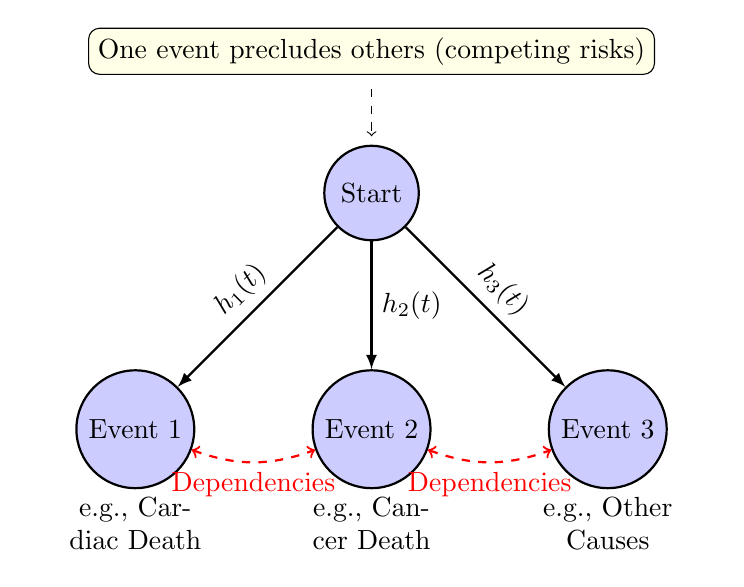
\begin{tikzpicture}[
        scale=1.2,
        event/.style={circle, draw, thick, fill=blue!20, minimum size=1.2cm, text centered},
        arrow/.style={->, >=latex, thick}
    ]
        \node[event] (start) at (0,0) {Start};
        \node[event] (event1) at (-2.5,-2.5) {Event 1};
        \node[event] (event2) at (0,-2.5) {Event 2};
        \node[event] (event3) at (2.5,-2.5) {Event 3};

        \draw[arrow] (start) -- (event1) node[midway, above, sloped] {$h_1(t)$};
        \draw[arrow] (start) -- (event2) node[midway, right] {$h_2(t)$};
        \draw[arrow] (start) -- (event3) node[midway, above, sloped] {$h_3(t)$};

        \node[text width=2.5cm, align=center] at (-2.5,-3.5) {e.g., Cardiac Death};
        \node[text width=2.5cm, align=center] at (0,-3.5) {e.g., Cancer Death};
        \node[text width=2.5cm, align=center] at (2.5,-3.5) {e.g., Other Causes};

        % Challenge annotations
        \draw[red, thick, dashed, <->] (event1) to[bend right=20] node[below] {Dependencies} (event2);
        \draw[red, thick, dashed, <->] (event2) to[bend right=20] node[below] {Dependencies} (event3);

        % Competing nature visualization
        \node[draw, rounded corners, fill=yellow!10, align=center] at (0,1.5) {One event precludes others (competing risks)};
        \draw[->, dashed] (0,1.1) -- (0,0.6);
    \end{tikzpicture}
    \caption{Competing risks structure, showing transitions from a starting state to multiple possible events, with dependencies between events.}
    \label{fig:mensa-competing-risks-diagram}
\end{figure}

\section{The Competing Risks Framework}

\subsection{Data Representation in Competing Risks}

In the competing risks setting, each subject can experience one of $J$ different event types. We observe a triplet of information for each subject $i$:

\begin{definitionbox}[title=Competing Risks Data Structure]
For each subject $i$, we observe:
\begin{itemize}
    \item $T_i$: The observed time (either event time or censoring time)
    \item $J_i \in \{1, 2, \ldots, J\}$: The event type (if an event occurred)
    \item $\delta_i \in \{0, 1\}$: Censoring indicator (1 if event observed, 0 if censored)
\end{itemize}

If $\delta_i = 0$ (censored), then $J_i$ is undefined as no event has been observed.
\end{definitionbox}

Table \ref{tab:competing-risks-data} shows an example dataset with competing risks. Note how censored subjects (rows 3 and 5) have no defined event type.

\begin{table}[htbp]
    \centering
    \caption{Example of competing risks data structure}
    \label{tab:competing-risks-data}
    \begin{tabular}{@{}cccc@{}}
        \toprule
        Subject & Time $T_i$ & Event Type $J_i$ & Indicator $\delta_i$ \\
        \midrule
        1 & 3.5 & 1 & 1 \\
        2 & 5.0 & 2 & 1 \\
        3 & 7.0 & -- & 0 \\
        4 & 2.3 & 3 & 1 \\
        5 & 4.2 & -- & 0 \\
        \bottomrule
    \end{tabular}
\end{table}

In this example:
\begin{itemize}
    \item Subject 1 experienced event type 1 at time 3.5
    \item Subject 2 experienced event type 2 at time 5.0
    \item Subject 3 was censored at time 7.0 without experiencing any event
    \item Subject 4 experienced event type 3 at time 2.3
    \item Subject 5 was censored at time 4.2 without experiencing any event
\end{itemize}

\subsection{Censoring in Competing Risks}

Censoring becomes more complex in the competing risks setting. We need to distinguish between:

\begin{itemize}
    \item \textbf{Administrative censoring}: The study ended before any event was observed
    \item \textbf{Competing event censoring}: A different event occurred, which precludes observation of the event of interest
\end{itemize}

\begin{figure}[htbp]
    \centering
    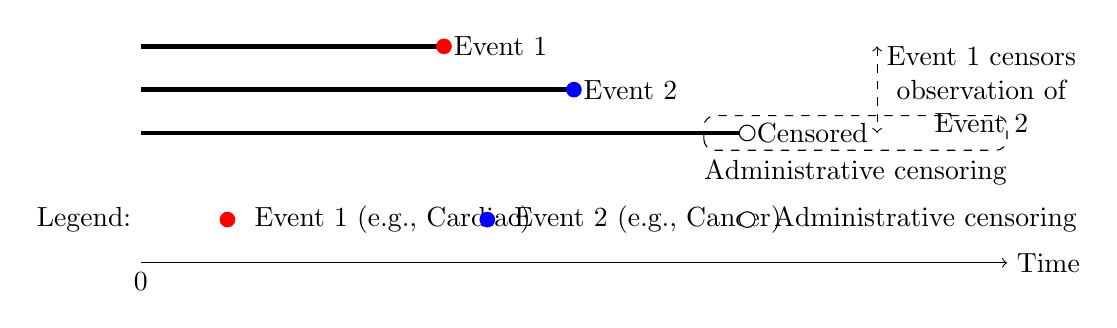
\begin{tikzpicture}[scale=1.1]
        % Timeline
        \draw[->] (0,0) -- (10,0) node[right] {Time};
        \draw (0,0) node[below] {0};

        % Patient 1: Event 1
        \draw[ultra thick, -] (0,2.5) -- (3.5,2.5);
        \draw (3.5,2.5) node[circle, fill=red, inner sep=2pt] {};
        \node[right] at (3.5,2.5) {Event 1};

        % Patient 2: Event 2
        \draw[ultra thick, -] (0,2) -- (5,2);
        \draw (5,2) node[circle, fill=blue, inner sep=2pt] {};
        \node[right] at (5,2) {Event 2};

        % Patient 3: Censored
        \draw[ultra thick, -] (0,1.5) -- (7,1.5);
        \draw (7,1.5) node[circle, draw, fill=white, inner sep=2pt] {};
        \node[right] at (7,1.5) {Censored};

        % Event types legend
        \node[left] at (0,0.5) {Legend:};
        \draw (1,0.5) node[circle, fill=red, inner sep=2pt] {};
        \node[right] at (1.2,0.5) {Event 1 (e.g., Cardiac)};
        \draw (4,0.5) node[circle, fill=blue, inner sep=2pt] {};
        \node[right] at (4.2,0.5) {Event 2 (e.g., Cancer)};
        \draw (7,0.5) node[circle, draw, fill=white, inner sep=2pt] {};
        \node[right] at (7.2,0.5) {Administrative censoring};

        % Annotations for censoring types
        \draw[<->, dashed] (8.5,2.5) -- (8.5,1.5) node[midway, right, align=center] {Event 1 censors\\observation of\\Event 2};
        \draw[dashed, rounded corners] (6.5,1.3) rectangle (10,1.7);
        \node[below] at (8.25,1.3) {Administrative censoring};
    \end{tikzpicture}
    \caption{Illustration of censoring in competing risks. The occurrence of Event 1 prevents observing whether Event 2 would have occurred, creating a form of informative censoring specific to competing risks.}
    \label{fig:competing-risks-censoring}
\end{figure}

This distinction is crucial because competing event censoring is informative for the event of interest, unlike standard administrative censoring which is typically assumed to be non-informative. In Figure \ref{fig:competing-risks-censoring}, for Patient 1, we'll never know if or when Event 2 would have occurred because Event 1 happened first.

\section{Key Functions in Competing Risks}

To properly analyze competing risks data, we need to define several key functions that extend traditional survival analysis concepts.

\subsection{Cause-Specific Hazard Function}

\begin{definitionbox}[title=Cause-Specific Hazard]
The cause-specific hazard for event $j$ represents the instantaneous risk of experiencing event $j$ at time $t$, given survival (no events of any type) up to time $t$:

\begin{equation}
h_j(t) = \lim_{\Delta t \to 0} \frac{P(t \leq T < t + \Delta t, J = j | T \geq t)}{\Delta t}
\end{equation}
\end{definitionbox}

The cause-specific hazard can be interpreted as the rate at which event $j$ occurs at time $t$ among subjects who have not yet experienced any event. Each event type has its own hazard function, and these functions can have different shapes.

\begin{figure}[htbp]
    \centering
    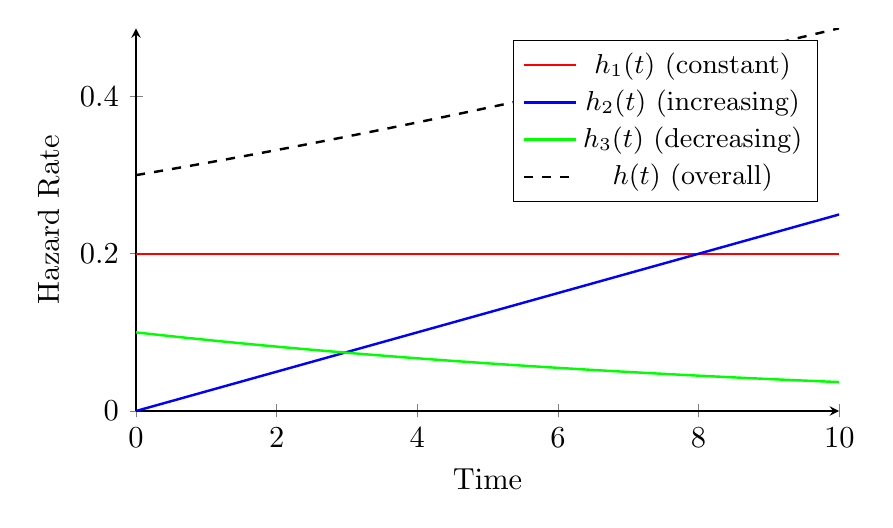
\begin{tikzpicture}[scale=1.1]
        % Coordinate system
        \begin{axis}[
            width=0.8\textwidth,
            height=6cm,
            xlabel={Time},
            ylabel={Hazard Rate},
            axis lines=left,
            domain=0:10,
            samples=100,
            legend pos=north east,
            legend style={font=\small}
        ]
            % Independent cause-specific hazards
            \addplot[red, thick] {0.2};
            \addplot[blue, thick] {0.05*(x/2)};
            \addplot[green, thick] {0.1*exp(-0.1*x)};
            % Total hazard
            \addplot[black, thick, dashed] {0.2+0.05*(x/2)+0.1*exp(-0.1*x)};
            \legend{$h_1(t)$ (constant), $h_2(t)$ (increasing), $h_3(t)$ (decreasing), $h(t)$ (overall)}
        \end{axis}
    \end{tikzpicture}
    \caption{Cause-specific hazard functions for three different event types. Note how each event can have a distinct hazard pattern (constant, increasing, or decreasing over time).}
    \label{fig:cause-specific-hazards}
\end{figure}

Figure \ref{fig:cause-specific-hazards} shows three different cause-specific hazard functions:
\begin{itemize}
    \item Event 1: Constant hazard (exponential distribution)
    \item Event 2: Increasing hazard (e.g., Weibull with shape parameter > 1)
    \item Event 3: Decreasing hazard (e.g., Weibull with shape parameter < 1)
\end{itemize}

The overall hazard function $h(t)$ is the sum of all cause-specific hazards:

\begin{equationbox}
\begin{equation}
h(t) = \sum_{j=1}^{J} h_j(t)
\end{equation}
\end{equationbox}

\subsection{Overall Survival Function}

The overall survival function represents the probability of not experiencing any event up to time $t$. It depends on all cause-specific hazards:

\begin{equationbox}[title=Overall Survival Function]
\begin{equation}
S(t) = P(T > t) = \exp\left(-\sum_{j=1}^{J} \int_0^t h_j(u) du\right) = \exp\left(-\sum_{j=1}^{J} H_j(t)\right)
\end{equation}

where $H_j(t) = \int_0^t h_j(u) du$ is the cumulative hazard for event $j$.
\end{equationbox}

This equation shows how the overall survival is affected by all event types. If any cause-specific hazard increases, the overall survival decreases more rapidly. The survival function can be factorized as the product of survival functions specific to each event type, if we were hypothetically able to remove other competing risks:

\begin{equation}
S(t) = \exp(-H_1(t)) \cdot \exp(-H_2(t)) \cdot \ldots \cdot \exp(-H_J(t))
\end{equation}

\subsection{Cumulative Incidence Function}

The Cumulative Incidence Function (CIF) is central to competing risks analysis. Unlike in standard survival, we need a separate CIF for each event type.

\begin{definitionbox}[title=Cumulative Incidence Function]
The CIF for event $j$ represents the probability of experiencing event $j$ by time $t$:

\begin{equation}
F_j(t) = P(T \leq t, J = j) = \int_0^t h_j(u) S(u) du
\end{equation}
\end{definitionbox}

The CIF accounts for the competing nature of risks by incorporating the overall survival function. At any time point, the sum of all CIFs plus the overall survival equals 1:

\begin{equation}
S(t) + \sum_{j=1}^{J} F_j(t) = 1
\end{equation}

\begin{figure}[htbp]
    \centering
    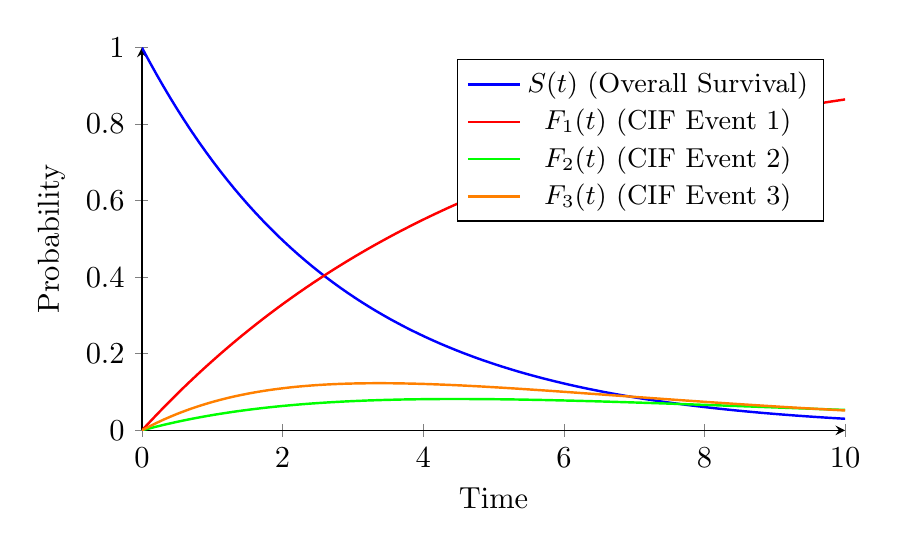
\begin{tikzpicture}[scale=1.1]
        \begin{axis}[
            width=0.8\textwidth,
            height=6cm,
            xlabel={Time},
            ylabel={Probability},
            axis lines=left,
            domain=0:10,
            samples=100,
            legend pos=north east,
            legend style={font=\small},
            ymin=0, ymax=1
        ]
            % Overall survival
            \addplot[blue, thick] {exp(-0.2*x-0.05*x-0.1*x)};
            % Event 1 CIF
            \addplot[red, thick] {1-exp(-0.2*x)};
            % Event 2 CIF
            \addplot[green, thick] {(1-exp(-0.05*x))*exp(-0.2*x)};
            % Event 3 CIF
            \addplot[orange, thick] {(1-exp(-0.1*x))*exp(-0.2*x-0.05*x)};
            \legend{$S(t)$ (Overall Survival), $F_1(t)$ (CIF Event 1), $F_2(t)$ (CIF Event 2), $F_3(t)$ (CIF Event 3)}
        \end{axis}
    \end{tikzpicture}
    \caption{Overall survival function and cause-specific cumulative incidence functions (CIFs) for three competing events. Note how all CIFs plus the survival function sum to 1 at any time point.}
    \label{fig:survival-cif}
\end{figure}

\subsection{Sub-Density Function}

The sub-density function for event $j$ is the derivative of the corresponding CIF:

\begin{equationbox}[title=Sub-Density Function]
\begin{equation}
f_j(t) = \frac{d}{dt}F_j(t) = h_j(t) S(t)
\end{equation}
\end{equationbox}

This represents the probability density of experiencing event $j$ at exactly time $t$. It equals the cause-specific hazard multiplied by the overall survival probability, capturing the joint effect of the instantaneous risk and the probability of having survived all events up to that time.

\section{Traditional Approaches to Competing Risks}

Before introducing MENSA, let's briefly review traditional methods for analyzing competing risks data.

\subsection{Cause-Specific Cox Models}

The most common approach is to fit separate Cox proportional hazards models for each event type:

\begin{equationbox}[title=Cause-Specific Cox Model]
\begin{equation}
h_j(t|\mathbf{x}) = h_{0j}(t) \exp(\boldsymbol{\beta}_j^T \mathbf{x})
\end{equation}

where $h_{0j}(t)$ is the baseline hazard for event $j$, and $\boldsymbol{\beta}_j$ are the coefficients for event $j$.
\end{equationbox}

This approach:
\begin{itemize}
    \item Treats each event type as a separate modeling problem
    \item Assumes proportional hazards for each cause-specific hazard
    \item Does not model dependencies between event types
    \item Requires separate models for each event of interest
\end{itemize}

\subsection{Fine-Gray Model}

The Fine-Gray model directly models the subdistribution hazard:

\begin{equationbox}[title=Fine-Gray Model]
\begin{equation}
h_j^{sub}(t|\mathbf{x}) = h_{0j}^{sub}(t) \exp(\boldsymbol{\gamma}_j^T \mathbf{x})
\end{equation}

where $h_j^{sub}(t) = -\frac{d\log(1-F_j(t))}{dt}$ is the subdistribution hazard.
\end{equationbox}

The Fine-Gray model:
\begin{itemize}
    \item Focuses on the CIF rather than the cause-specific hazard
    \item Allows direct modeling of cumulative incidence
    \item Also assumes proportional hazards (but for the subdistribution hazard)
    \item Requires separate models for each event type
\end{itemize}

\begin{notebox}
Both cause-specific Cox models and Fine-Gray models are semi-parametric and don't model the full joint distribution of events. They also don't naturally incorporate dependencies between event types or leverage neural networks for complex covariate relationships.
\end{notebox}

In the next section, we'll introduce the MENSA framework, which addresses these limitations through a parametric mixture approach combined with deep learning.

\section{The MENSA Framework}

\subsection{Core Conceptual Innovation}

MENSA builds on the DSM framework by extending it to handle multiple competing events. The key conceptual innovations include:

\begin{itemize}
    \item Using a mixture of parametric distributions for each event type
    \item Sharing representation learning across event types
    \item Modeling dependencies between events through shared latent space
    \item Maintaining flexible hazard shapes for each event
    \item Learning event-specific and shared risk factors
\end{itemize}

\begin{figure}[htbp]
    \centering
    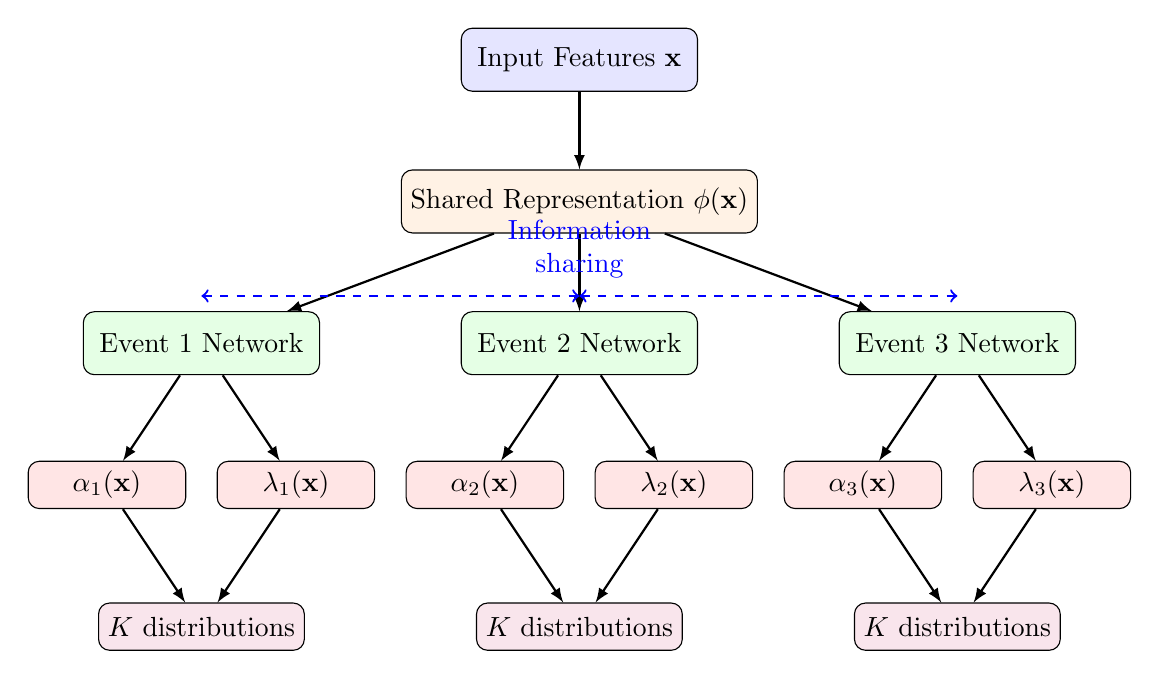
\begin{tikzpicture}[
        scale=1.2,
        box/.style={draw, rounded corners, minimum width=3cm, minimum height=0.8cm, text centered},
        param/.style={draw, rounded corners, minimum width=2cm, minimum height=0.6cm, text centered},
        arrow/.style={->, >=latex, thick}
    ]
        % Input layer
        \node[box, fill=blue!10] (input) at (0,0) {Input Features $\mathbf{x}$};
        
        % Shared representation
        \node[box, fill=orange!10] (shared) at (0,-1.5) {Shared Representation $\phi(\mathbf{x})$};
        
        % Event-specific networks
        \node[box, fill=green!10] (net1) at (-4,-3) {Event 1 Network};
        \node[box, fill=green!10] (net2) at (0,-3) {Event 2 Network};
        \node[box, fill=green!10] (net3) at (4,-3) {Event 3 Network};
        
        % Distribution parameters for each event
        \node[param, fill=red!10] (alpha1) at (-5,-4.5) {$\alpha_1(\mathbf{x})$};
        \node[param, fill=red!10] (lambda1) at (-3,-4.5) {$\lambda_1(\mathbf{x})$};
        
        \node[param, fill=red!10] (alpha2) at (-1,-4.5) {$\alpha_2(\mathbf{x})$};
        \node[param, fill=red!10] (lambda2) at (1,-4.5) {$\lambda_2(\mathbf{x})$};
        
        \node[param, fill=red!10] (alpha3) at (3,-4.5) {$\alpha_3(\mathbf{x})$};
        \node[param, fill=red!10] (lambda3) at (5,-4.5) {$\lambda_3(\mathbf{x})$};
        
        % Mixture components (distributions)
        \node[box, fill=purple!10, minimum width=2cm, minimum height=0.6cm] (dist1) at (-4,-6) {$K$ distributions};
        \node[box, fill=purple!10, minimum width=2cm, minimum height=0.6cm] (dist2) at (0,-6) {$K$ distributions};
        \node[box, fill=purple!10, minimum width=2cm, minimum height=0.6cm] (dist3) at (4,-6) {$K$ distributions};
        
        % Connections
        \draw[arrow] (input) -- (shared);
        \draw[arrow] (shared) -- (net1);
        \draw[arrow] (shared) -- (net2);
        \draw[arrow] (shared) -- (net3);
        
        \draw[arrow] (net1) -- (alpha1);
        \draw[arrow] (net1) -- (lambda1);
        \draw[arrow] (net2) -- (alpha2);
        \draw[arrow] (net2) -- (lambda2);
        \draw[arrow] (net3) -- (alpha3);
        \draw[arrow] (net3) -- (lambda3);
        
        \draw[arrow] (alpha1) -- (dist1);
        \draw[arrow] (lambda1) -- (dist1);
        \draw[arrow] (alpha2) -- (dist2);
        \draw[arrow] (lambda2) -- (dist2);
        \draw[arrow] (alpha3) -- (dist3);
        \draw[arrow] (lambda3) -- (dist3);
        
        % Information sharing annotation
        \draw[<->, dashed, blue, thick] (-4,-2.5) -- (0,-2.5);
        \draw[<->, dashed, blue, thick] (0,-2.5) -- (4,-2.5);
        \node[blue, text width=3cm, align=center] at (0,-2) {Information sharing};
    \end{tikzpicture}
    \caption{MENSA architecture showing the flow from input features through shared representation to event-specific networks and ultimately to the parameterization of the mixture distributions for each event type.}
    \label{fig:mensa-architecture}
\end{figure}

\subsection{Mathematical Formulation}

Let's formalize the MENSA framework mathematically. For a subject with covariates $\mathbf{x}$, we model the cause-specific hazard for each event type $j \in \{1, 2, \ldots, J\}$ as a mixture of parametric distributions:

\begin{equationbox}[title=MENSA Cause-Specific Hazard]
\begin{equation}
h_j(t|\mathbf{x}) = \sum_{k=1}^{K} w_{jk}(\mathbf{x}) \cdot h_{jk}(t|\alpha_{jk}(\mathbf{x}), \lambda_{jk}(\mathbf{x}))
\end{equation}

where:
\begin{itemize}
    \item $h_{jk}(t|\alpha_{jk}, \lambda_{jk})$ is the hazard function for the $k$-th component of event type $j$
    \item $w_{jk}(\mathbf{x})$ are the mixture weights for event $j$, with $\sum_{k=1}^{K} w_{jk}(\mathbf{x}) = 1$
    \item $\alpha_{jk}(\mathbf{x})$ and $\lambda_{jk}(\mathbf{x})$ are the shape and scale parameters of the distributions
\end{itemize}
\end{equationbox}

Typically, MENSA uses Weibull distributions for the mixture components:

\begin{equation}
h_{jk}(t|\alpha_{jk}, \lambda_{jk}) = \frac{\alpha_{jk}}{\lambda_{jk}} \left(\frac{t}{\lambda_{jk}}\right)^{\alpha_{jk}-1}
\end{equation}

The overall survival function is:

\begin{equation}
S(t|\mathbf{x}) = \exp\left(-\sum_{j=1}^{J} \int_0^t h_j(u|\mathbf{x}) \, du\right)
\end{equation}

And the cumulative incidence function for event $j$ is:

\begin{equation}
F_j(t|\mathbf{x}) = \int_0^t h_j(u|\mathbf{x}) \cdot S(u|\mathbf{x}) \, du
\end{equation}

\subsection{Neural Network Architecture}

MENSA implements the above formulation using neural networks to learn the parameters:

\begin{enumerate}
    \item \textbf{Shared representation network:} $\phi(\mathbf{x})$ maps input features to a shared latent space
    \item \textbf{Event-specific networks:} Map from the shared representation to event-specific parameters
    \item \textbf{Distribution parameter networks:} Output the shape and scale parameters for each event and mixture component
\end{enumerate}

The sharing of the representation $\phi(\mathbf{x})$ enables information transfer across event types, while event-specific networks capture the unique characteristics of each event type.

\begin{notebox}[title=Advantages of the MENSA Architecture]
The MENSA architecture offers several advantages:
\begin{itemize}
    \item \textbf{Flexibility:} The mixture of distributions allows for complex, multi-modal hazard shapes
    \item \textbf{Information sharing:} Common risk factors can be learned from the pooled data across events
    \item \textbf{Event-specific modeling:} Each event has its own dedicated parameters
    \item \textbf{End-to-end learning:} All parameters are learned jointly via maximum likelihood
    \item \textbf{Dependency modeling:} The shared representation captures correlations between event risks
\end{itemize}
\end{notebox}

\section{Training and Optimization}

\subsection{Likelihood Function}

MENSA is trained by maximizing the likelihood of the observed data. The likelihood function for competing risks data needs to account for both event occurrences and censoring:

\begin{equationbox}[title=MENSA Likelihood Function]
\begin{equation}
\mathcal{L}(\theta) = \prod_{i: \delta_i=1} f_{J_i}(T_i|\mathbf{x}_i, \theta) \prod_{i: \delta_i=0} S(T_i|\mathbf{x}_i, \theta)
\end{equation}

where:
\begin{itemize}
    \item $\theta$ represents all model parameters
    \item $f_j(t|\mathbf{x}, \theta) = h_j(t|\mathbf{x}, \theta) S(t|\mathbf{x}, \theta)$ is the sub-density function for event $j$
    \item $S(t|\mathbf{x}, \theta)$ is the overall survival function
\end{itemize}
\end{equationbox}

Taking the logarithm, we get the log-likelihood:

\begin{equation}
\ell(\theta) = \sum_{i: \delta_i=1} \log h_{J_i}(T_i|\mathbf{x}_i, \theta) + \sum_{i=1}^{n} \log S(T_i|\mathbf{x}_i, \theta)
\end{equation}

The first term involves the cause-specific hazard for observed events, while the second term includes the overall survival function for all subjects (both events and censored).

\subsection{Optimization Techniques}

Training MENSA involves several optimization considerations:

\begin{itemize}
    \item \textbf{Parameter initialization:} Careful initialization of distribution parameters is crucial for stable training
    \item \textbf{Gradient-based optimization:} Typically using Adam or similar optimizers
    \item \textbf{Regularization:} L1/L2 regularization to prevent overfitting
    \item \textbf{Handling data imbalance:} When some event types are rare, balancing techniques may be needed
    \item \textbf{Early stopping:} Based on validation performance
\end{itemize}

\subsection{Avoiding Numerical Issues}

MENSA's training can face numerical stability challenges:

\begin{itemize}
    \item \textbf{Vanishing/exploding gradients:} Addressed through gradient clipping
    \item \textbf{Distribution parameter constraints:} All shape and scale parameters must be positive (typically enforced through softplus activation)
    \item \textbf{Loss scaling:} The log-likelihood may need scaling for stable gradients
    \item \textbf{Mixture component collapse:} Regularization techniques to prevent mixture components from collapsing
\end{itemize}

\begin{examplebox}[title=Code Example: MENSA Parameter Constraints]
\begin{verbatim}
# Ensuring positivity of Weibull parameters
alpha = nn.Softplus()(alpha_logits) + 0.01  # Shape parameter
lambda_ = nn.Softplus()(lambda_logits) + 0.01  # Scale parameter

# Ensuring mixture weights sum to 1
weights = nn.Softmax(dim=-1)(weight_logits)  # Mixture weights
\end{verbatim}
\end{examplebox}

\section{Inference and Risk Prediction}

\subsection{Risk Predictions with MENSA}

MENSA enables several types of risk predictions:

\begin{enumerate}
    \item \textbf{Overall survival probability:} $S(t|\mathbf{x})$
    \item \textbf{Cumulative incidence of event $j$:} $F_j(t|\mathbf{x})$
    \item \textbf{Cause-specific hazard of event $j$:} $h_j(t|\mathbf{x})$
    \item \textbf{Time to event density for event $j$:} $f_j(t|\mathbf{x})$
    \item \textbf{Conditional event probability:} $P(J=j|T=t, \mathbf{x}) = \frac{h_j(t|\mathbf{x})}{\sum_{j'=1}^{J} h_{j'}(t|\mathbf{x})}$
\end{enumerate}

These predictions can be computed for individual subjects, allowing for personalized risk assessment.

\subsection{Uncertainty Quantification}

MENSA provides several approaches to quantify uncertainty in predictions:

\begin{itemize}
    \item \textbf{Direct parameterization:} The mixture components naturally model uncertainty in the event timing
    \item \textbf{Epistemic uncertainty:} Can be estimated using ensembling or Monte Carlo dropout
    \item \textbf{Aleatoric uncertainty:} Captured through the inherent variability of the parametric distributions
    \item \textbf{Confidence intervals:} Can be constructed via bootstrapping or analytical approximations
\end{itemize}

\subsection{Interpreting MENSA Models}

Interpreting the complex MENSA model can be approached in several ways:

\begin{itemize}
    \item \textbf{Feature importance:} Using permutation-based or gradient-based importance measures
    \item \textbf{Partial dependence plots:} Showing the relationship between specific features and predicted risks
    \item \textbf{Shapley values:} Quantifying the contribution of each feature to predictions
    \item \textbf{Distribution visualization:} Plotting the learned mixture distributions for each event type
\end{itemize}

\begin{figure}[htbp]
    \centering
    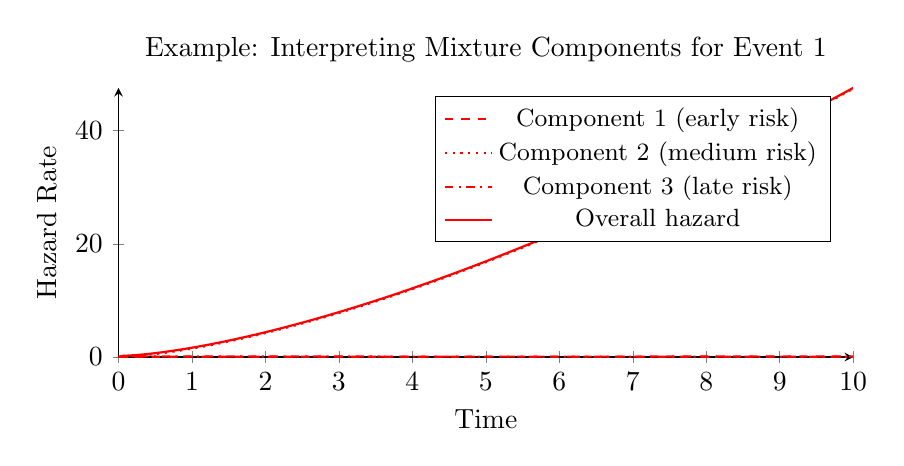
\begin{tikzpicture}
        \begin{axis}[
            width=0.9\textwidth,
            height=5cm,
            xlabel={Time},
            ylabel={Hazard Rate},
            axis lines=left,
            domain=0:10,
            samples=150,
            legend pos=north east,
            legend style={font=\small},
            title={Example: Interpreting Mixture Components for Event 1}
        ]
            % Components of the mixture
            \addplot[red, thick, dashed] {0.1*(1.2/2)*(x/2)^(1.2-1)};
            \addplot[red, thick, dotted] {0.6*(2.5/1)*(x/1)^(2.5-1)};
            \addplot[red, thick, dashdotted] {0.3*(0.8/3)*(x/3)^(0.8-1)};
            % Overall event hazard
            \addplot[red, thick] {0.1*(1.2/2)*(x/2)^(1.2-1) + 0.6*(2.5/1)*(x/1)^(2.5-1) + 0.3*(0.8/3)*(x/3)^(0.8-1)};
            \legend{Component 1 (early risk), Component 2 (medium risk), Component 3 (late risk), Overall hazard}
        \end{axis}
    \end{tikzpicture}
    \caption{Interpretation of mixture components for an event's hazard function. Each component might represent a different risk sub-group or risk mechanism.}
    \label{fig:mixture-interpretation}
\end{figure}

\section{Applications of MENSA}

\subsection{Medical Applications}

MENSA is particularly valuable in medical settings with multiple possible outcomes:

\begin{itemize}
    \item \textbf{Cancer progression:} Modeling competing risks of cancer-specific death versus other causes
    \item \textbf{Cardiovascular diseases:} Predicting different types of cardiovascular events (heart attack, stroke, etc.)
    \item \textbf{Organ transplantation:} Modeling risks of rejection, infection, and other complications
    \item \textbf{Multiple disease progression:} For patients with comorbidities facing multiple potential health events
\end{itemize}

\subsection{Industrial Applications}

In industrial settings, MENSA can model competing failure modes:

\begin{itemize}
    \item \textbf{Manufacturing:} Predicting different types of component failures
    \item \textbf{Energy systems:} Modeling various failure modes in power generation equipment
    \item \textbf{Transportation:} Predictive maintenance accounting for multiple failure types
    \item \textbf{Infrastructure:} Risk assessment for different types of structural failures
\end{itemize}

\subsection{Business Applications}

MENSA can also be applied to business scenarios with competing events:

\begin{itemize}
    \item \textbf{Customer churn:} Modeling different reasons for customer attrition
    \item \textbf{Credit risk:} Predicting different types of default or delinquency
    \item \textbf{Marketing:} Modeling competing conversion types
    \item \textbf{Employee turnover:} Predicting different reasons for employee departures
\end{itemize}

\section{Future Directions}

MENSA opens several promising directions for future research:

\begin{itemize}
    \item \textbf{Recurrent events:} Extending to scenarios where events can occur multiple times
    \item \textbf{Semi-competing risks:} Handling scenarios where some events preclude others but not vice versa
    \item \textbf{Time-varying covariates:} Incorporating dynamic features that change over time
    \item \textbf{Multi-state extensions:} Moving beyond competing risks to full multi-state models
    \item \textbf{Causal inference:} Integrating causal frameworks to estimate intervention effects
    \item \textbf{Treatment recommendation:} Using MENSA to guide personalized treatment decisions
\end{itemize}

\section{Summary}

Multi-Event Neural Survival Analysis (MENSA) extends the DSM framework to handle competing risks scenarios, providing a powerful approach for modeling complex time-to-event data with multiple possible outcomes. Key advantages include:

\begin{itemize}
    \item Flexible modeling of cause-specific hazards through mixture distributions
    \item Sharing information across event types while maintaining event-specific modeling
    \item Capturing dependencies between different event types
    \item End-to-end learning of all parameters via maximum likelihood
    \item Comprehensive risk predictions and uncertainty quantification
\end{itemize}

By combining the strengths of parametric survival modeling with deep learning, MENSA offers a promising framework for addressing complex survival analysis problems in healthcare, industry, and business applications.